\documentclass[11pt,letterpaper]{article}
\usepackage[lmargin=1in,rmargin=1in,tmargin=1in,bmargin=1in]{geometry}
\usepackage{../style/homework}
\usepackage{../style/commands}
\setbool{quotetype}{true} % True: Side; False: Under
\setbool{hideans}{false} % Student: True; Instructor: False

% -------------------
% Content
% -------------------
\begin{document}

\homework{1: Due 09/28}{Clark Kent is Superman's critique on the whole human race.}{Bill, Kill Bill}

% Problem 1
\problem{10} Two relations, $F$ and $G$, are represented below. Are either $F$ or $G$ functions? Explain. 
	\[
	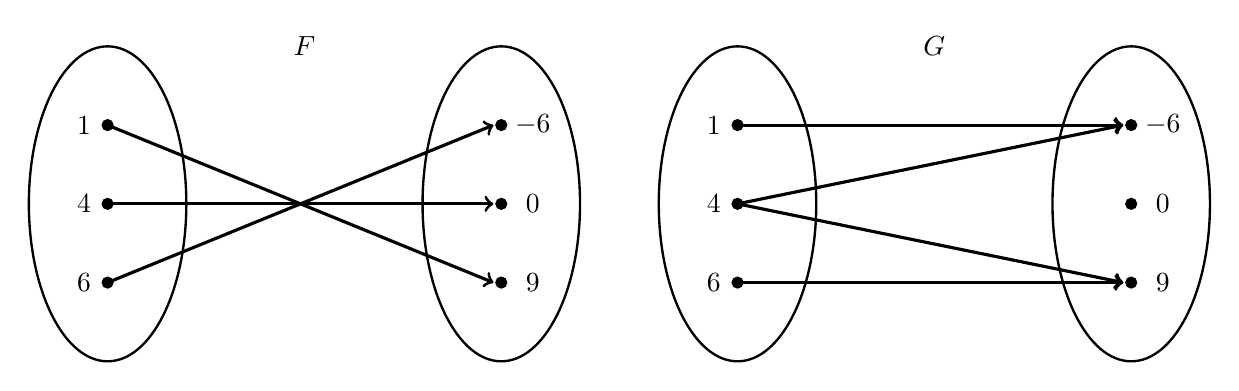
\begin{tikzpicture}
	\node at (2.5,2) {$F$};
	% Ellipses
	\draw[line width=0.03cm] (0,0) circle (1 and 2);
	\draw[line width=0.03cm] (5,0) circle (1 and 2);
	
	% Nodes
	\draw[fill=black] (0,1) circle (0.07);
	\draw[fill=black] (0,0) circle (0.07);
	\draw[fill=black] (0,-1) circle (0.07);
	
	\draw[fill=black] (5,1) circle (0.07);
	\draw[fill=black] (5,0) circle (0.07);
	\draw[fill=black] (5,-1) circle (0.07);
	
	% Arrow
	\draw[line width=0.04cm,->] (0,1) -- (4.9,-1);
	\draw[line width=0.04cm,->] (0,0) -- (4.9,0);
	\draw[line width=0.04cm,->] (0,-1) -- (4.9,1);
	
	% Labels
	\node at (-0.3,1) {$1$};
	\node at (-0.3,0) {$4$};
	\node at (-0.3,-1) {$6$};
	
	\node at (5.4,1) {$-6$};
	\node at (5.4,0) {$0$};
	\node at (5.4,-1) {$9$};
	
	\tikzset{shift={(8,0)}}
	%
	\node at (2.5,2) {$G$};
	% Ellipses
	\draw[line width=0.03cm] (0,0) circle (1 and 2);
	\draw[line width=0.03cm] (5,0) circle (1 and 2);
	
	% Nodes
	\draw[fill=black] (0,1) circle (0.07);
	\draw[fill=black] (0,0) circle (0.07);
	\draw[fill=black] (0,-1) circle (0.07);
	
	\draw[fill=black] (5,1) circle (0.07);
	\draw[fill=black] (5,0) circle (0.07);
	\draw[fill=black] (5,-1) circle (0.07);
	
	% Arrow
	\draw[line width=0.04cm,->] (0,1) -- (4.9,1);
	\draw[line width=0.04cm,->] (0,0) -- (4.9,1);
	\draw[line width=0.04cm,->] (0,0) -- (4.9,-1);
	\draw[line width=0.04cm,->] (0,-1) -- (4.9,-1);
	
	% Labels
	\node at (-0.3,1) {$1$};
	\node at (-0.3,0) {$4$};
	\node at (-0.3,-1) {$6$};
	
	\node at (5.4,1) {$-6$};
	\node at (5.4,0) {$0$};
	\node at (5.4,-1) {$9$};
	\end{tikzpicture}
	\] \pspace

\sol {\itshape The relation $F$ is a function---for every input there is only one output. However, the relation $G$ is not a function. For instance, the input 4 in the domain has two possible outputs---namely $-6$ and $9$.}



\newpage



% Problem 2
\problem{10} Given the following tables, do $f(x)$ and $g(x)$ represent functions? Explain. 
	\begin{table}[!ht]
	\centering \setlength\arrayrulewidth{0.02cm}
	\begin{tabular}{c|ccc|c} 
	$x$ & $f(x)$ & \hspace{2cm} & $x$ & $g(x)$ \\ \cline{1-2} \cline{4-5}
	$1$ & $3$ && $1$ & $4$ \\
	$2$ & $6$ && $2$ & $1$ \\
	$3$ & $9$ && $3$ & $4$ \\
	$4$ & $2$ && $4$ & $5$ \\
	$5$ & $5$ && $1$ & $3$  
	\end{tabular}
	\end{table} \pspace

\sol {\itshape The relation $f(x)$ is a function because for every input there is only one possible output. However, the relation $g(x)$ is not a function. The value 1 appears twice in the domain (which is not a problem). However, in these different appearances, the input 1 takes different values. Then for this input we have more than one possible output so that $g(x)$ is not a function. Note that the fact that $g(x)= 4$ for several values, i.e. $g(1)= 4$ and $g(3)= 4$, does not affect whether or not $g(x)$ is a function or not.}
	


\vfill
\newpage



% Problem 3
\problem{10} Does the formula $f(x):= 2.31x + 9.55$ give a function? Explain. If it is a function, describe its graph. \pspace

{\itshape The formula $f(x)$ is a function. For each input, we only have one possible output---namely, the one given by plugging $x$ into $2.31x + 9.55$ and following order of operations. Observe that $f(x)$ has the form $mx + b$ so that $f(x)$ is a linear function. Therefore, it's graph is a line.} \pvspace{2.1cm} 



% Problem 4
\problem{10} For each of the following, indicate whether the equation is a linear equation (T), or not (F). 
	\begin{enumerate}[(a)]
	\item \usol{0.7cm}{T}: $2x - 3y= 9$
	\item \usol{0.7cm}{F}: $2x^2 + 5y^2= 7$
	\item \usol{0.7cm}{T}: $x= 5$
	\item \usol{0.7cm}{T}: $x= 6- y$
	\item \usol{0.7cm}{F}: $y= x^2 + x + 1$
	\end{enumerate}



\vfill



% Problem 5
\problem{10} For each of the following, indicate whether the function is linear (T), or not (F). 
	\begin{enumerate}[(a)]
	\item \usol{0.7cm}{T}: $y= 2x + 1$
	\item \usol{0.7cm}{T}: $f(x)= 1 - 6x$
	\item \usol{0.7cm}{F}: $y= x ( 2x + 1)$
	\item \usol{0.7cm}{T}: $y= 2(x - 1)$
	\item \usol{0.7cm}{T}: $f(x)= \frac{1}{3}x - 9$
	\end{enumerate}



\vfill
\newpage



% Problem 6
\problem{10} Given the data in the table below, is it reasonable to say that the data is linear? Explain. 
	\begin{table}[!ht]
	\centering
	\begin{tabular}{c|c}
	$x$ & $f(x)$ \\ \hline
	$1$ & $4$ \\
	$2$ & $6$ \\
	$3$ & $8$ \\
	$4$ & $10$ \\
	$6$ & $12$ 
	\end{tabular}
	\end{table} \pspace

\sol {\itshape It is plausible to say that the data is linear. If the data were to be linear, the slope between the points would have to be constant. Rather than compute every possible slope, we compute only one---the one between the first two points:
	\[
	m= \dfrac{\Delta y}{\Delta x}= \dfrac{4 - 6}{1 - 2}= \dfrac{-2}{-1}= 2
	\]
Now if the data were to be linear, the slope between all the points must be 2. Because $m= \frac{\Delta y}{\Delta x}= \frac{2}{1}$, for every increase of 1 in $x$, we should see an increase of 2 in $y$. Notice this is the case for $x$ from 2 to 3, 3 to 4, but not 4 to 6. When $x$ goes from 4 to 6, $x$ has increased by 2 so that we should see an increase of $2(2)= 4$ in $y$; however, $y$ only increases by 2. Therefore, the data cannot be perfectly linear. 
}



\newpage



% Problem 7
\problem{10} Complete the following parts: 
\begin{enumerate}[(a)]
\item Find the equation of the line through the points $(1, -5)$ and $(-2, 13)$. \pspace
	\[
	m= \dfrac{\Delta y}{\Delta x}= \dfrac{-5 - 13}{1 - (-2)}= \dfrac{-18}{3}= - 6
	\]
	\[
	\begin{aligned}
	y&= mx + b \\
	y&= -6x + b \\
	-5&= -6(1) + b \\
	-5&= -6 + b \\
	b&= 1
	\end{aligned}
	\]
{\itshape Then the equation of the line is $y= -6x + 1$.} \pvspace{0.9cm}

\item What is the slope and $y$-intercept of the line from (a)? \pspace

{\itshape The slope of the line is $-6$ and the $y$-intercept is $(0, 1)$.} \pvspace{5.6cm}

\item Sketch the line from (a) as accurately as possible. 
	\[
	\fbox{
	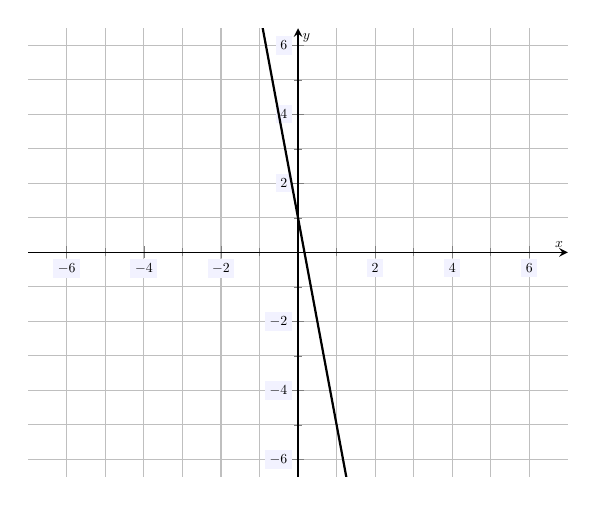
\begin{tikzpicture}[scale=1,every node/.style={scale=0.5}]
	\begin{axis}[
	grid=both,
	axis lines=middle,
	ticklabel style={fill=blue!5!white},
	xmin= -7, xmax=7,
	ymin= -6.5, ymax=6.5,
	xtick={-6,-4,-2,0,2,4,6},
	ytick={-6,-4,-2,0,2,4,6},
	minor tick = {-5,-3,...,5},
	xlabel=\(x\),ylabel=\(y\),
	]
	\addplot[thick, domain= -7:7] {-6*x + 1};
	\end{axis}
	\end{tikzpicture}
	}
	\]
\end{enumerate}



\newpage



% Problem 8
\problem{10} Consider the line given by $f(x)= 6x + 5$.
\begin{enumerate}[(a)]
\item Find the $y$-intercept for this line. \pspace
	\[
	f(0)= 6(0) + 5= 0 + 5= 5
	\]
{\itshape Therefore, the $y$-intercept is $(0, 5)$.} \pvspace{2.5cm}

\item Find the $x$-intercept for this line. \pspace
	\[
	\begin{aligned}
	f(x)&= 0 \\
	6x + 5&= 0 \\
	6x&= -5 \\
	x= -\dfrac{5}{6}
	\end{aligned}
	\]
{\itshape Therefore, the $x$-intercept is $(-5/6, 0)$.} \pvspace{0.5cm}

\item Is the point $(0, 1)$ on the line? Explain. \pspace

{\itshape We have $f(0)= 6(0) + 5= 0 + 5= 5$. Therefore, $(0, 5)$ is a point on the function but $(0, 1)$ cannot be. Alternatively, using the fact that $y= 6x + 5$, we can check if $(0, 1)$ satisfies this equation, but $1 \neq 6(0) + 5= 0 + 5= 5$ so that the point is not on the graph of $f(x)$.} \pvspace{2.6cm}

\item Is the point $(-1, -1)$ on the line? Explain. \pspace

{\itshape We have $f(-1)= 6(-1) + 5= -6 + 5= -1$ so that $(-1, -1)$ is a point on the line. Alternatively, we can check if $(-1, -1)$ satisfies the equation $y= 6x + 5$. Observe $-1= 6(-1)= -6 + 5= -1$ so that $(-1, -1)$ is on the graph of $f(x)$.}
\end{enumerate}


\end{document}